%-------------------------------------------------------------------------------
% PARTIE 1
%-------------------------------------------------------------------------------
Les fichiers informatiques présents dans cet article sont tous accessibles depuis le site d’activités informatiques de l’IREM Paris Nord : \href{http://www-irem.univ-paris13.fr/site_spip/spip.php?rubrique57}{Rubricamaths}
. L’utilisation de celui-ci permet un accès simple aux activités et permet d’individualiser le travail avec les élèves. En effet, vous y trouverez de nombreuses autres activités similaires à celles présentées avec des niveaux de difficultés graduelles.



\section{Les lignes droites}

%-------------------------------------------------------------------------------
\subsection{Pour commencer}

\subsubsection{Activité Papier : Figures sur papiers marqués}

L’élève doit reproduire le dessin présenté. Il ne peut utiliser comme seul instrument que la règle (non graduée). La seule obligation à respecter est que les points à relier sont des nœuds des papiers maillés, des points des papiers pointés.

\begin{multicols}{5}

  \begin{figure}[H]
    \centering
    \fbox{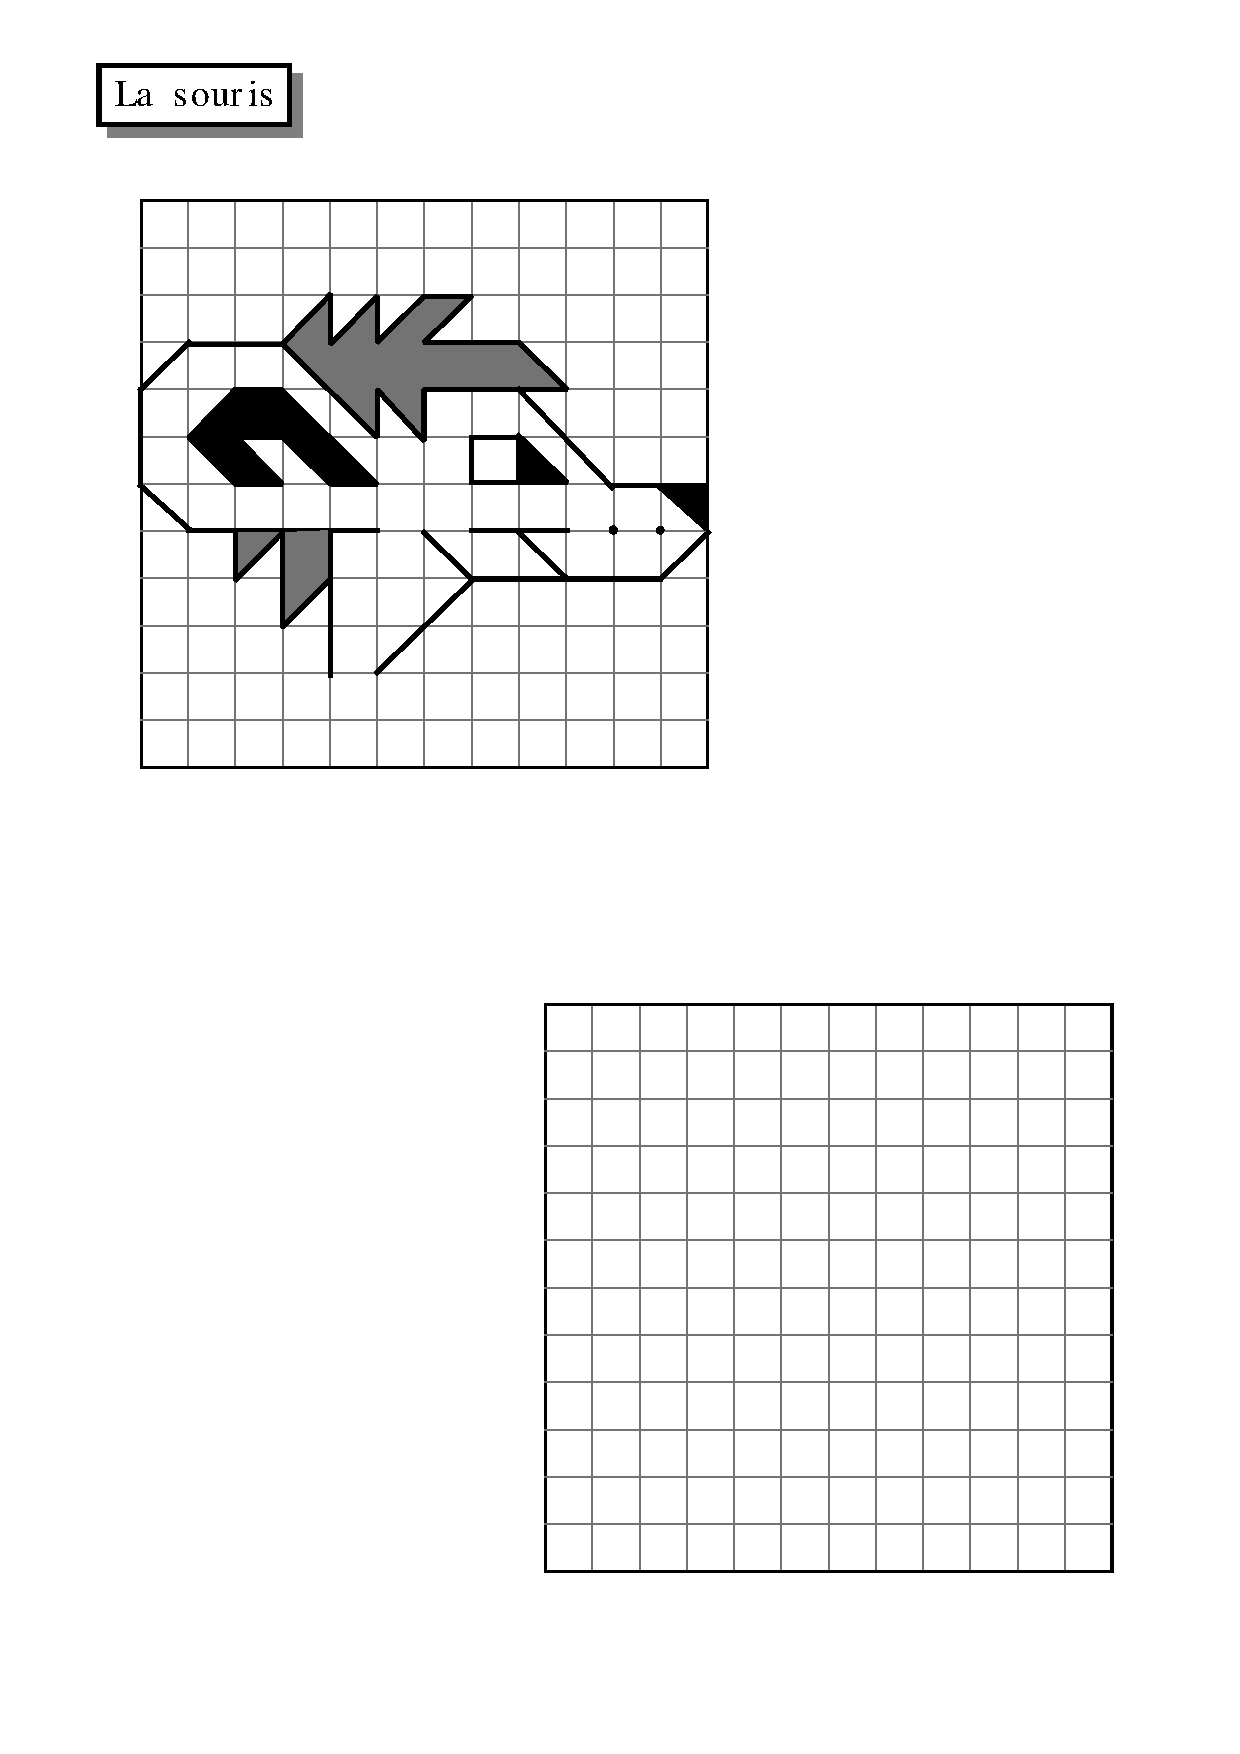
\includegraphics[width=0.8\linewidth]{sources/pages/1.1.1/1-souris.pdf}}
    \caption{\hyperref[souris]{Souris}}
  \end{figure}

  \begin{figure}[H]
    \centering
    \fbox{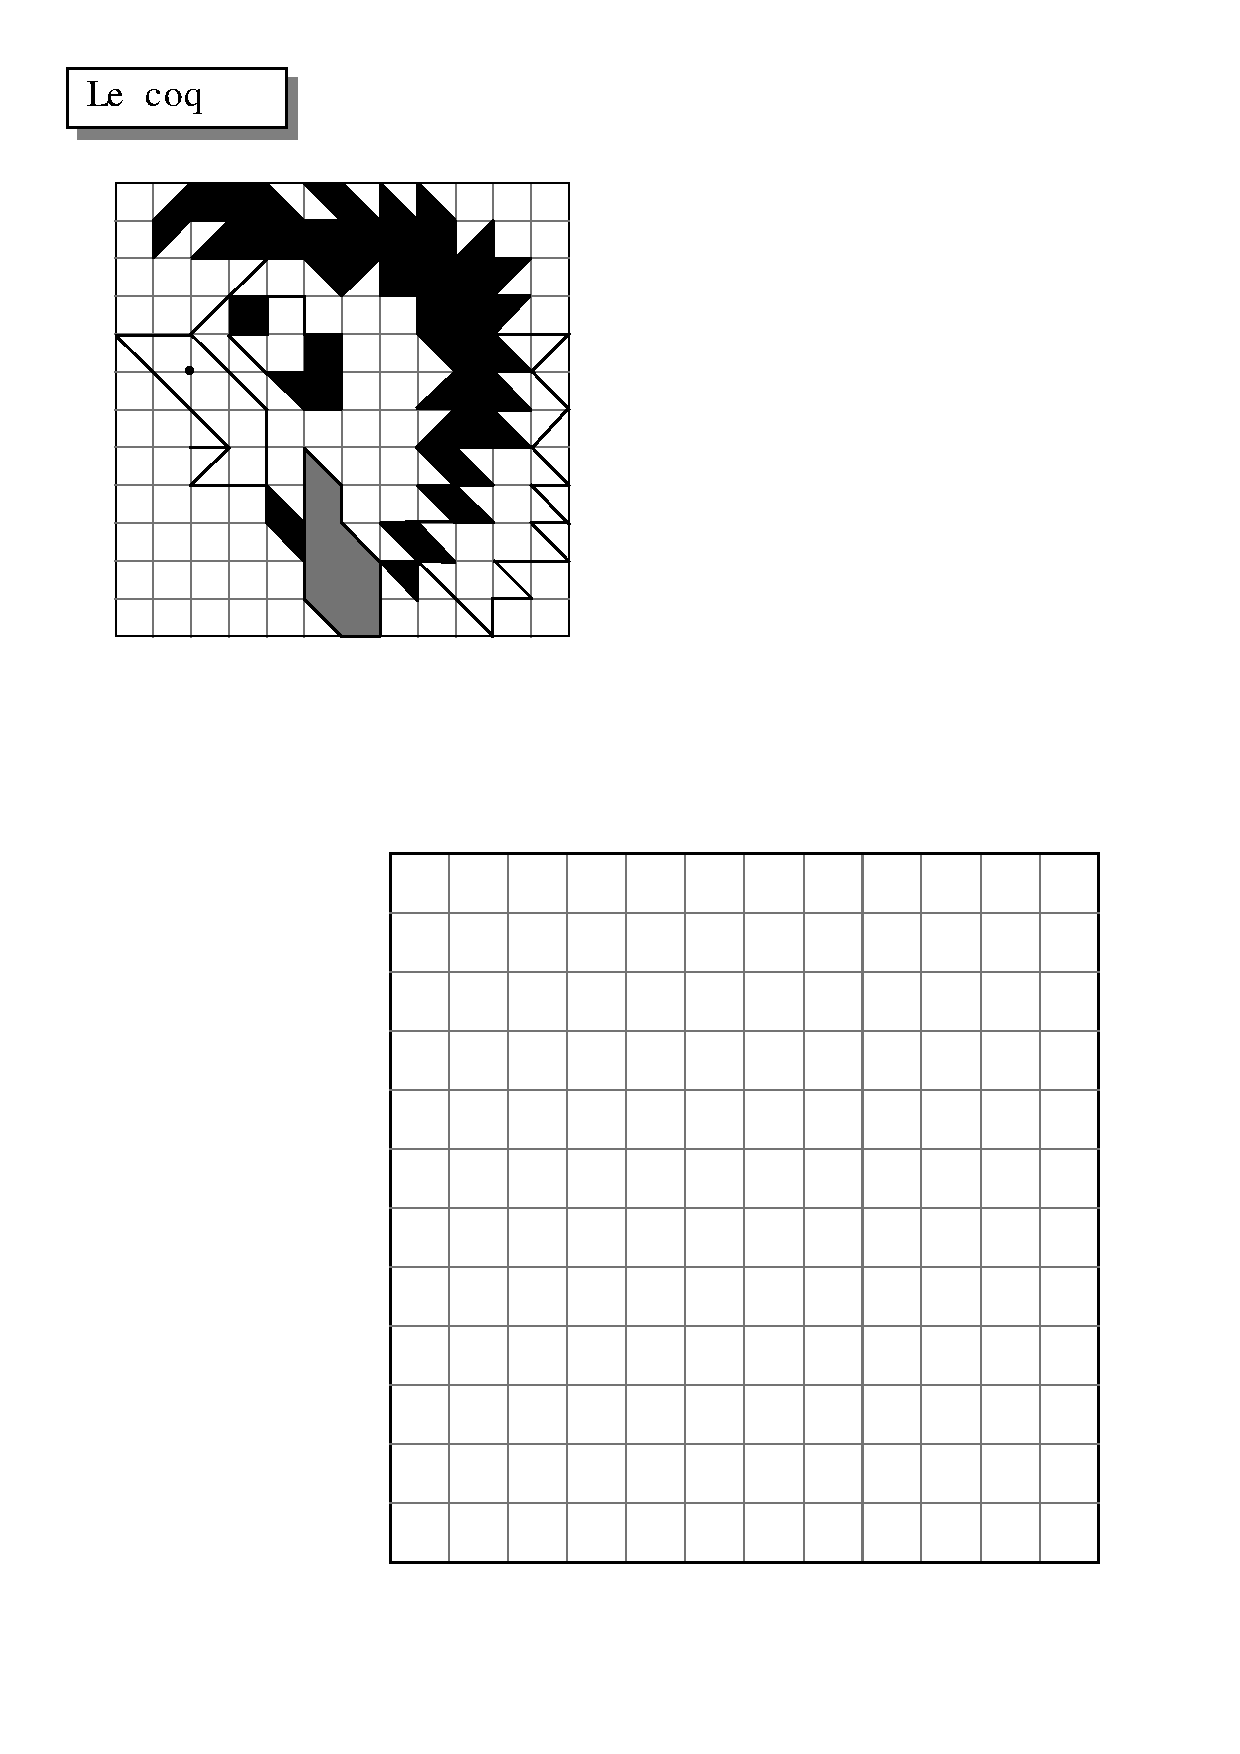
\includegraphics[width=0.8\linewidth]{sources/pages/1.1.1/2-coq.pdf}}
    \caption{\hyperref[coq]{Coq}}
  \end{figure}

  \begin{figure}[H]
    \centering
    \fbox{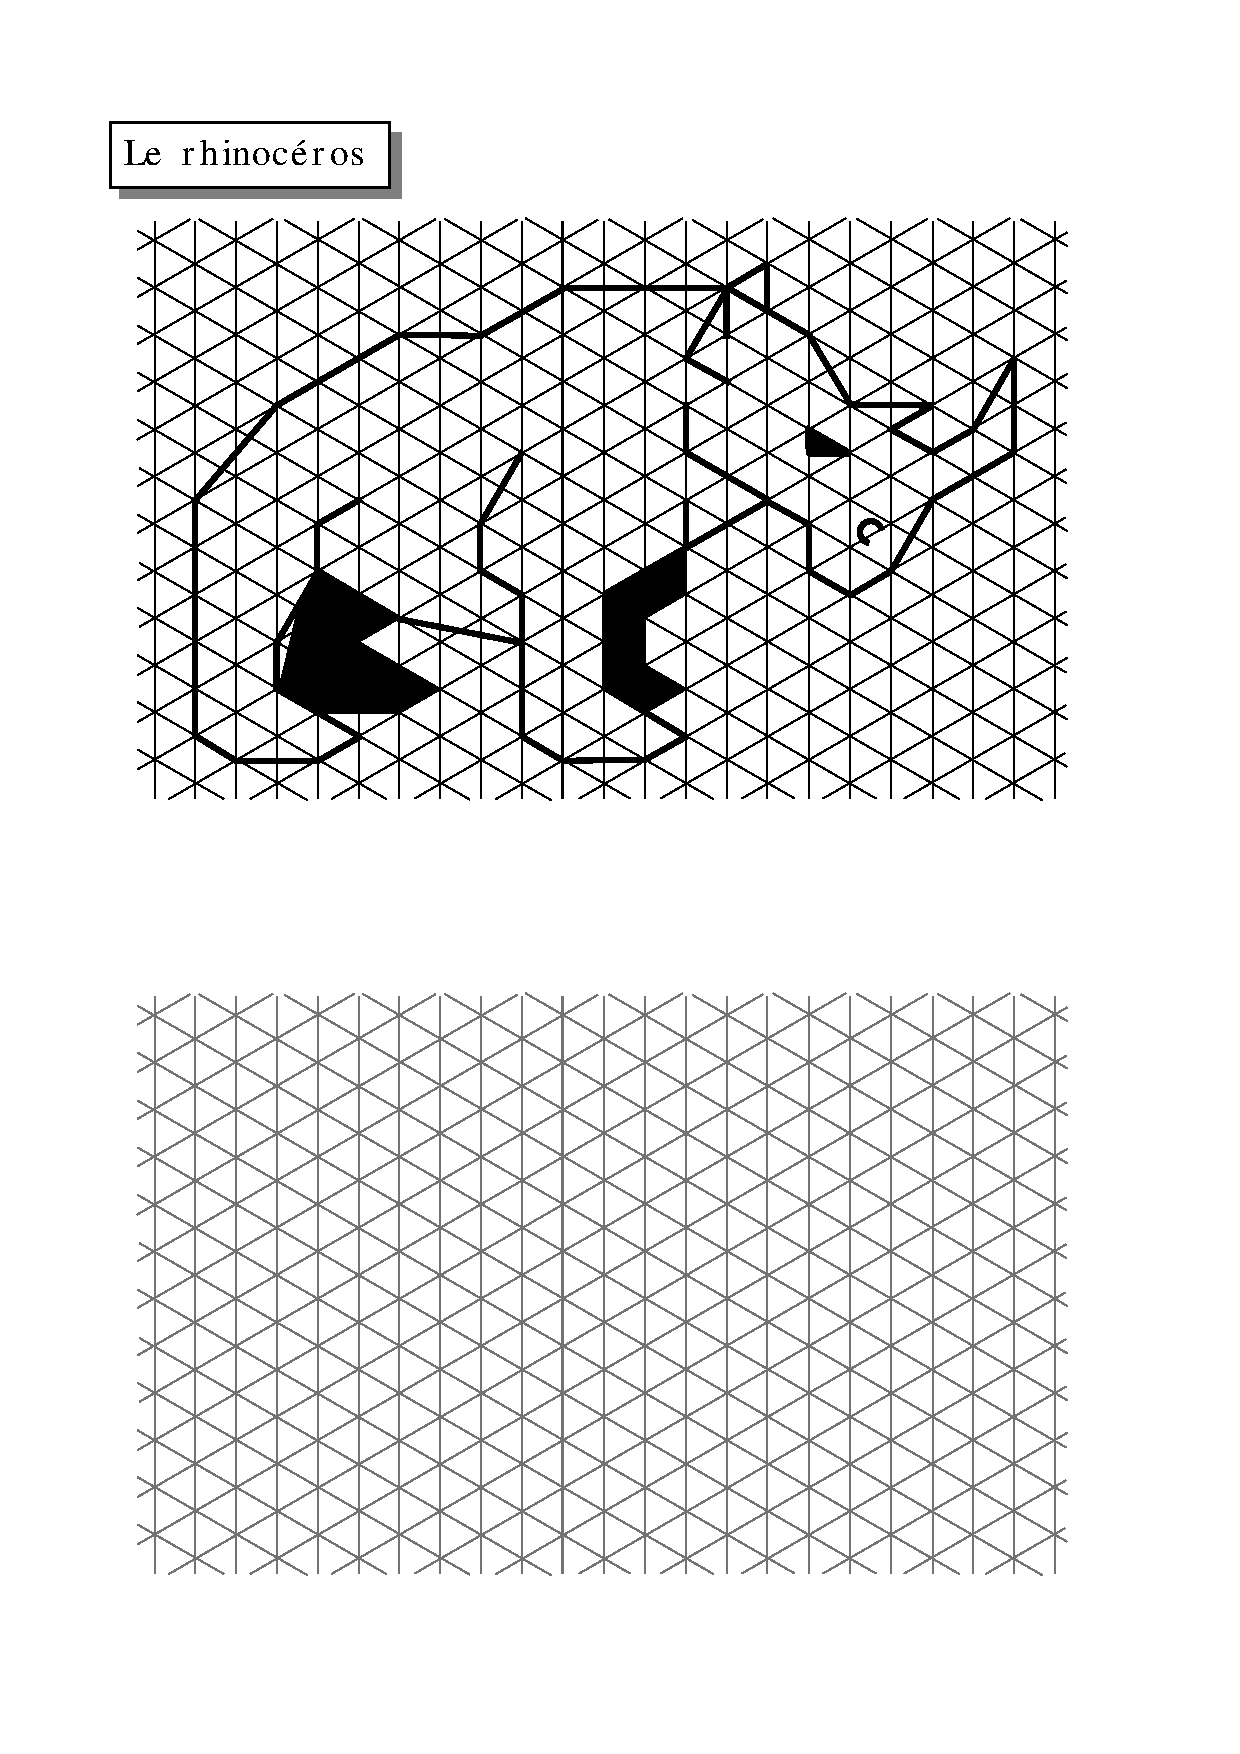
\includegraphics[width=0.8\linewidth]{sources/pages/1.1.1/3-rhino.pdf}}
    \caption{\hyperref[rhino]{Rhino}}
  \end{figure}

  \begin{figure}[H]
    \centering
    \fbox{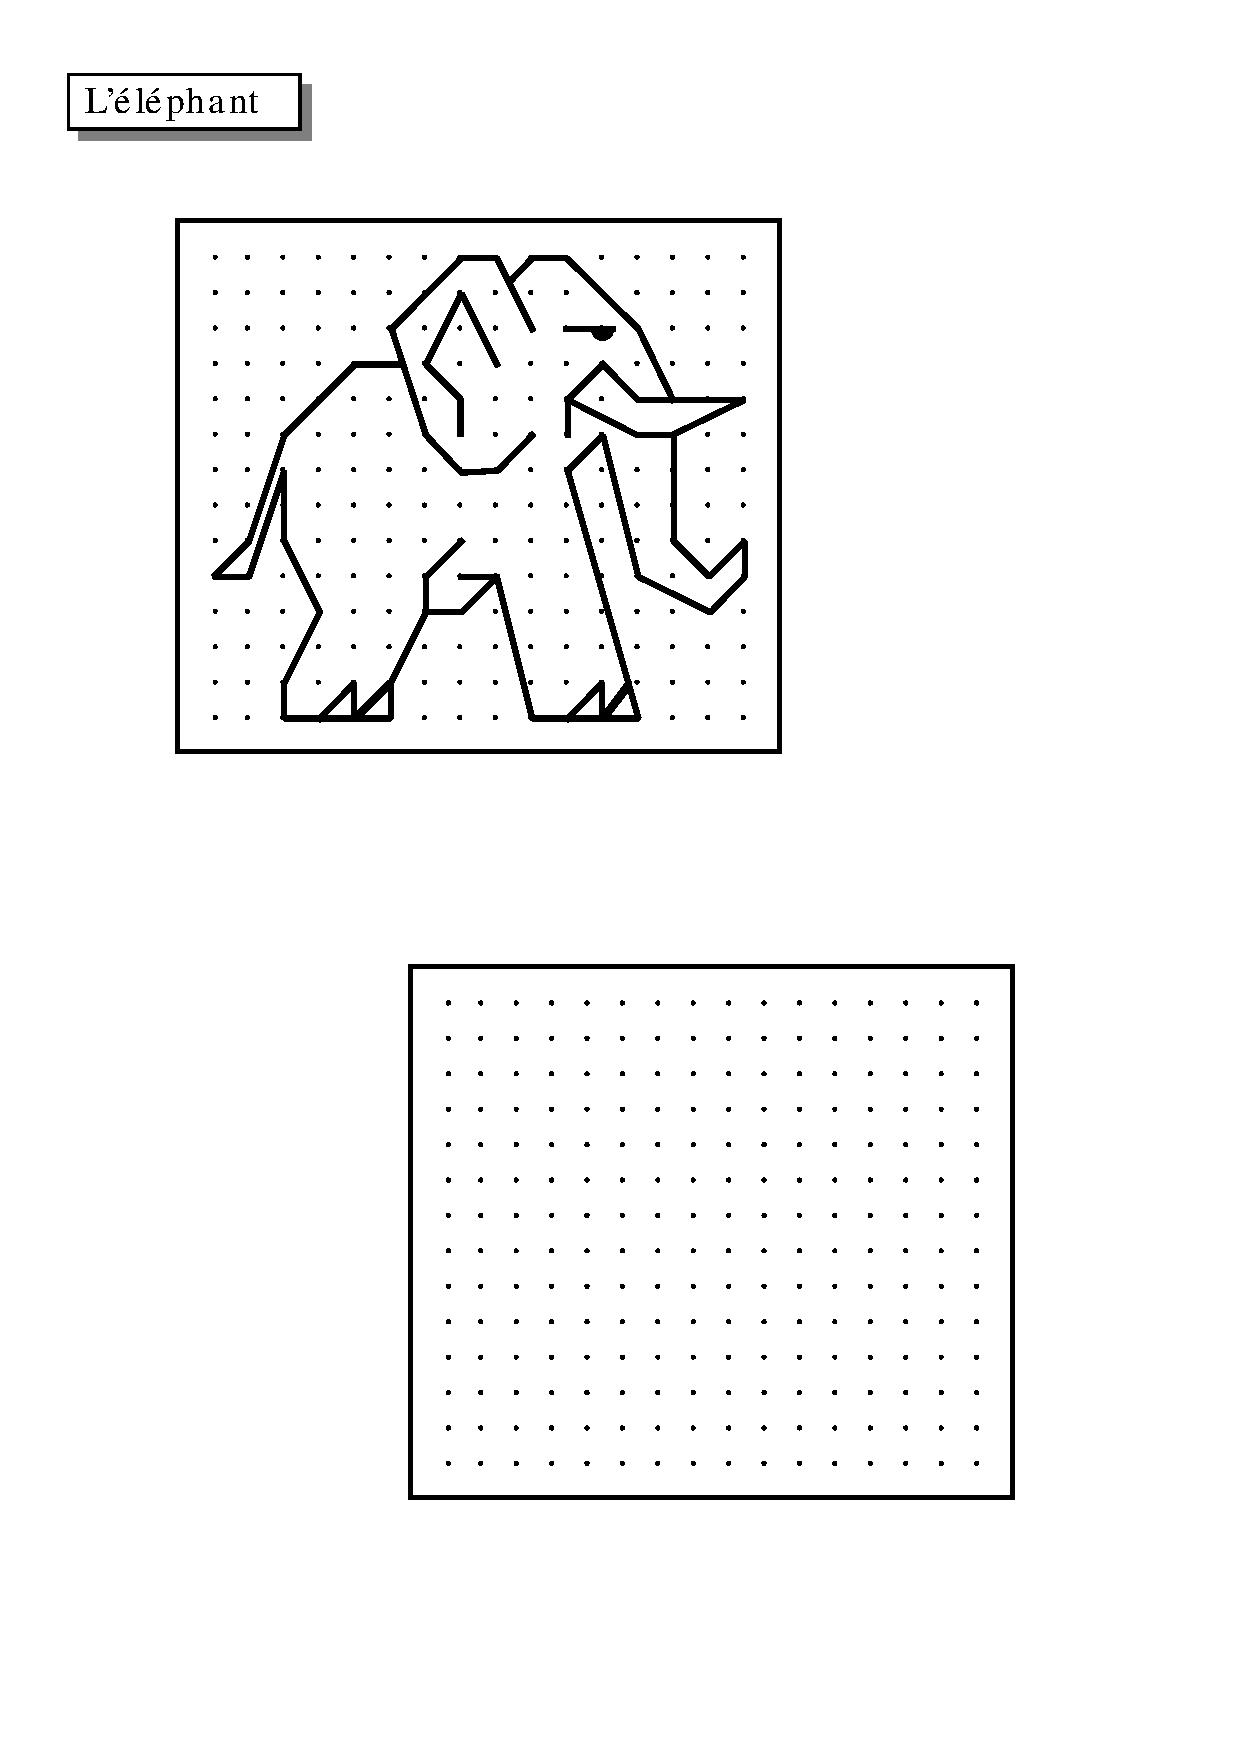
\includegraphics[width=0.8\linewidth]{sources/pages/1.1.1/4-elephant.pdf}}
    \caption{\hyperref[elephant]{Elephant}}
  \end{figure}

  \begin{figure}[H]
    \centering
    \fbox{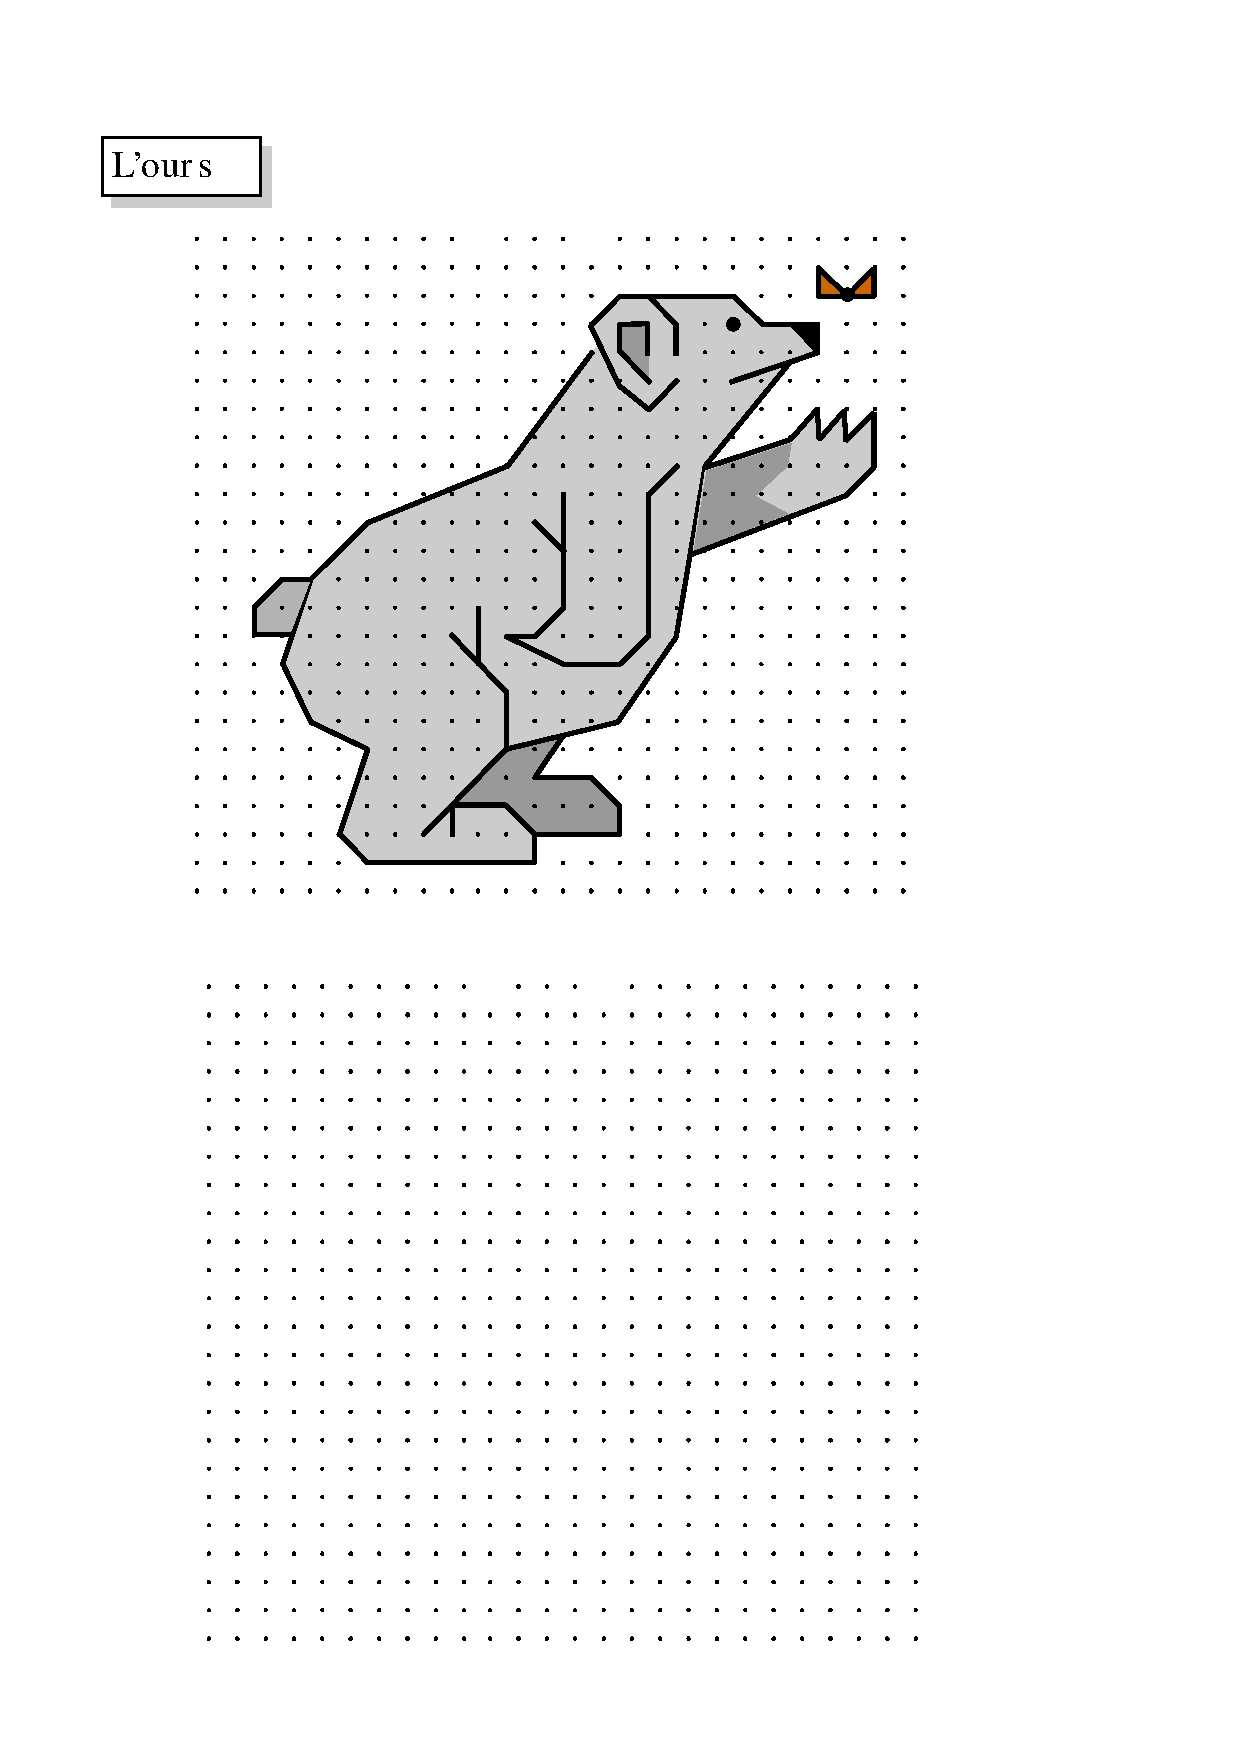
\includegraphics[width=0.8\linewidth]{sources/pages/1.1.1/5-ours.pdf}}
    \caption{\hyperref[ours]{Ours}}
  \end{figure}
\end{multicols}

On peut moduler le nombre de dessins à proposer en fonction de l’adresse manuelle des élèves, de leur capacité de soin, de leur bonne compréhension des consignes, etc.

La plupart de ces dessins peuvent être proposés comme travail à la maison.

\textit{Pour trouver d’autres dessins à réaliser, se reporter aux brochures de l’Irem Paris-Nord, en particulier \og Papiers-Crayons \fg{}.}

\subsubsection{ Activité Géogébra : Découvrir Géogébra}

En salle informatique, avec un vidéo-projecteur (si c’est possible), faire découvrir aux élèves :
\begin{itemize}
  \item les outils de la barre de menu \og Lignes droites \fg{} : pointer, point, droite, segment, demi-droite, polygone, nommer, cacher/montrer, couleur et remplir ;
  \item les actions indispensables : déplacer un objet, effacer un objet, etc.
\end{itemize}

Ensuite, la liste des savoir-faire indispensables est donnée aux élèves qui découvrent et expérimentent à leur rythme ces différentes commandes sur un fichier géogebra vide comprenant uniquement les outils nécessaire.
L’expérience montre que 20 min de découverte et 20 min de libre utilisation sont nécessaires et suffisantes pour la bonne prise en main du logiciel.

\begin{multicols}{2}

  \begin{figure}[H]
    \centering
    \fbox{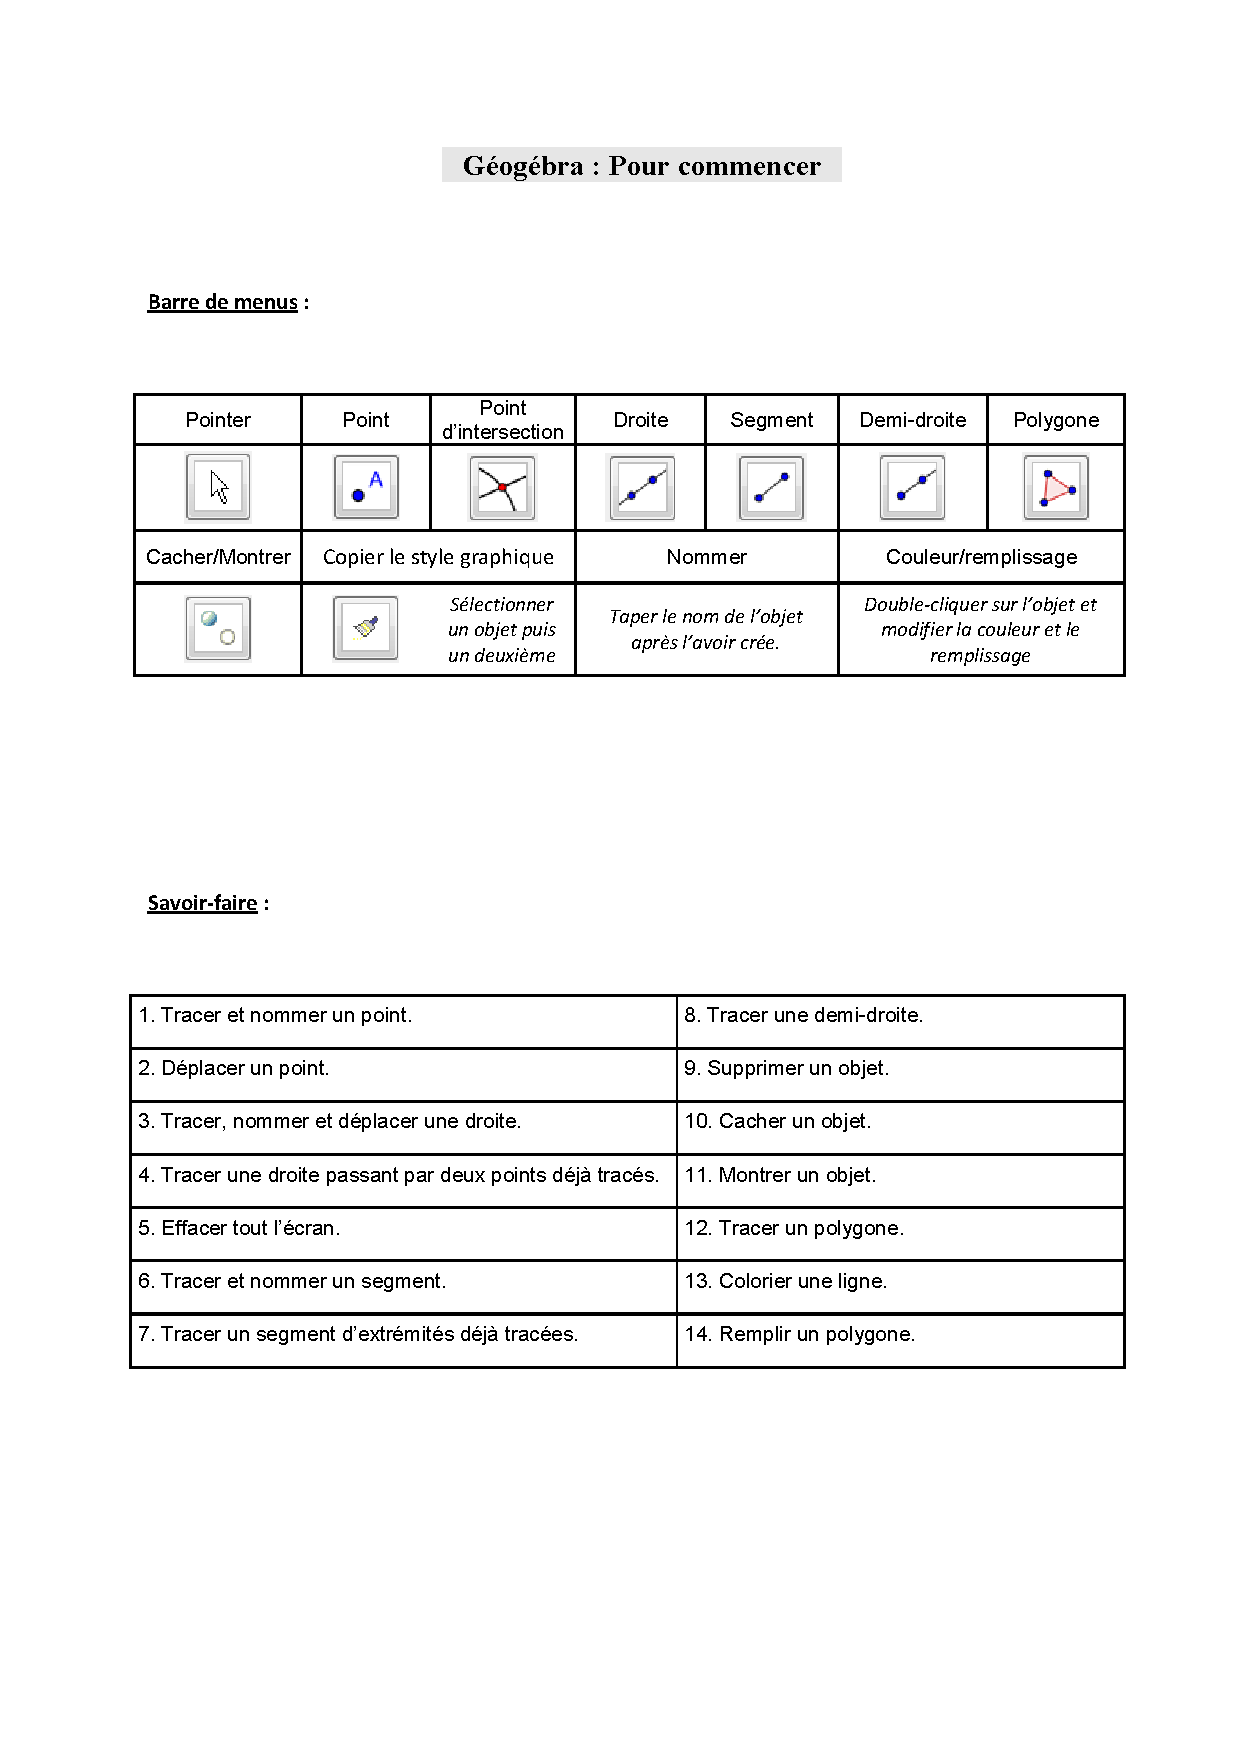
\includegraphics[width=0.4\linewidth]{sources/pages/1.1.2/pour_commencer.pdf}}
    \caption{\hyperref[geo-commencer]{Pour Commencer}}
  \end{figure}

  \begin{figure}[H]
    \centering
    \fbox{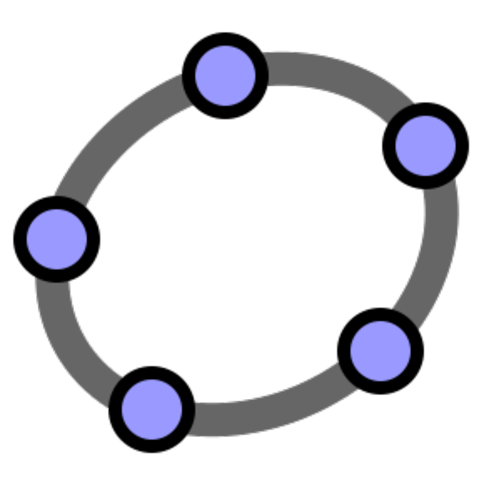
\includegraphics[width=0.3\linewidth]{sources/icones/geogebra.pdf}}
    \caption{\href{http://www-irem.univ-paris13.fr/site_spip/IMG/ggb/menu_lignes_droites-3.ggb}{Menu lignes droites}}
  \end{figure}
\end{multicols}

%-------------------------------------------------------------------------------
\subsection{Droites et segments}

\subsubsection{Activité Papier : Reproduire une figure}

L’élève doit reproduire le dessin présenté à partir des éléments de départ qui lui sont donnés. Il ne peut utiliser comme seul instrument que la règle ( non graduée). La seule obligation à respecter et qu’aucun des points à relier n’est pris au hasard.

\begin{figure}[H]
  \centering
   \fbox{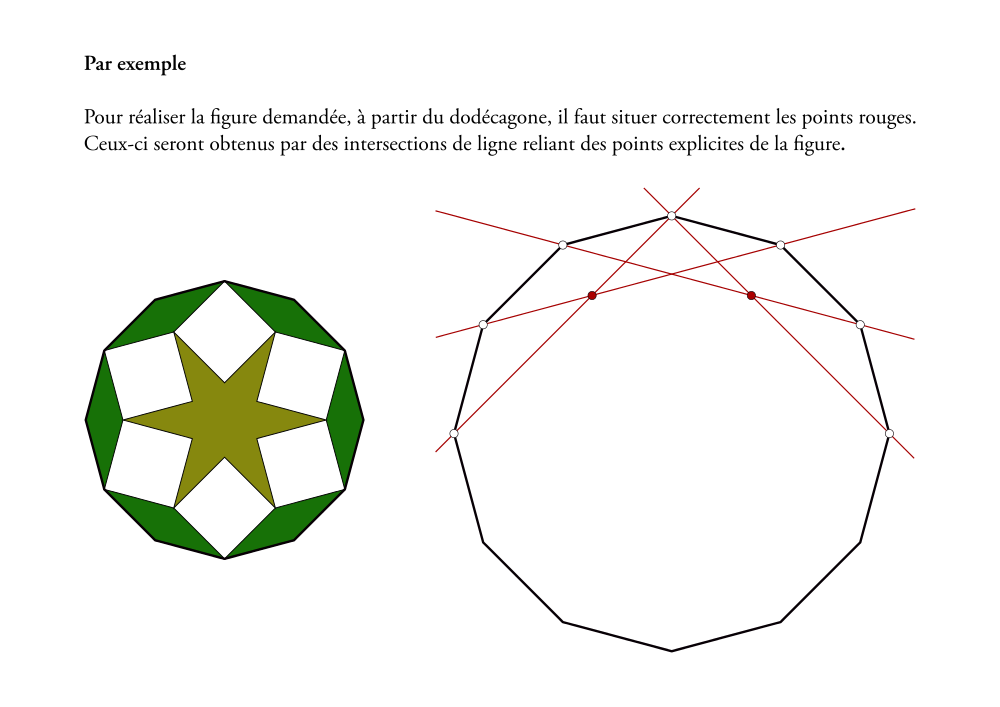
\includegraphics[width=0.6\linewidth]{sources/img/1-im2.png}}
\end{figure}

La série suivante de dessin papier est proposée aux élèves :

\begin{multicols}{3}

  \begin{figure}[H]
    \centering
    \fbox{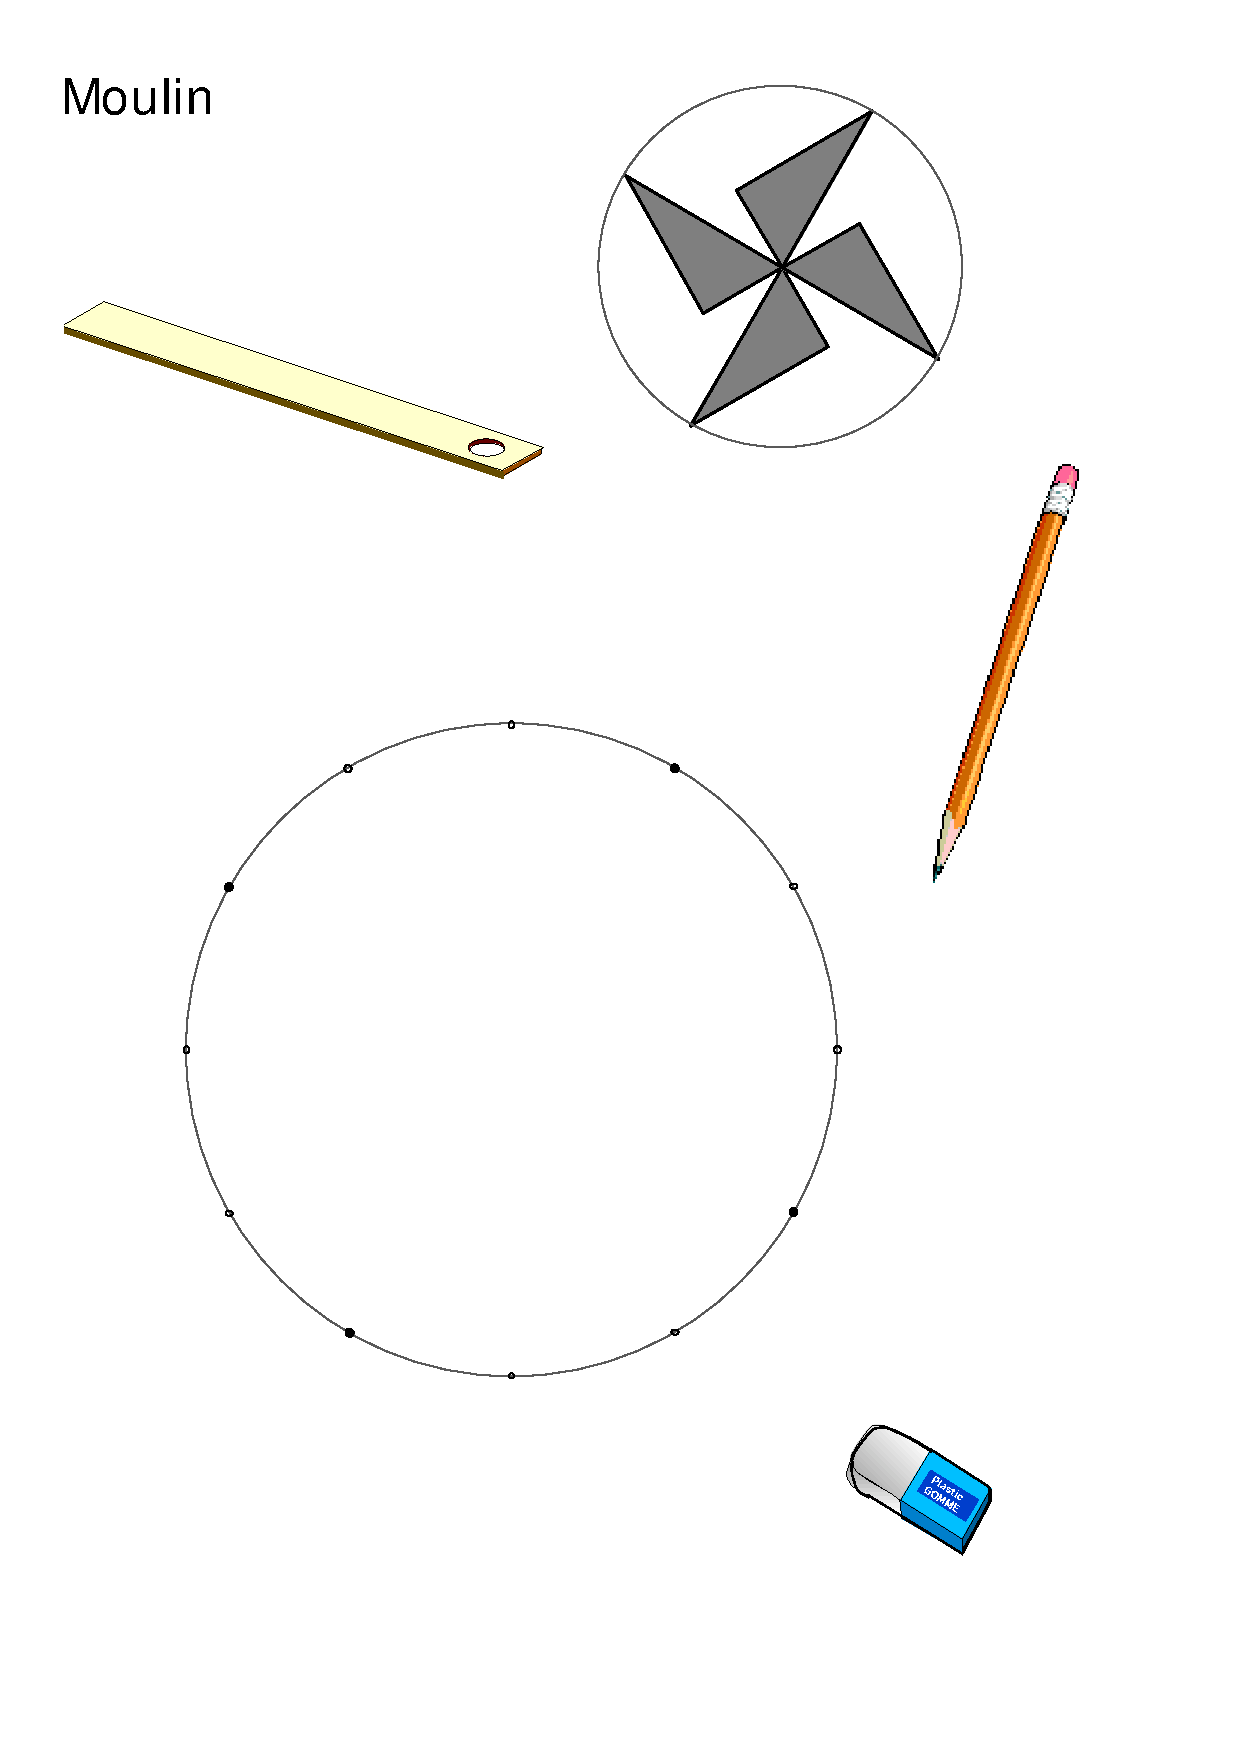
\includegraphics[width=0.3\linewidth]{sources/pages/1.2.1/1-moulinette.pdf}}
    \caption{\hyperref[moulinette]{Moulinette}}
  \end{figure}

  \begin{figure}[H]
    \centering
    \fbox{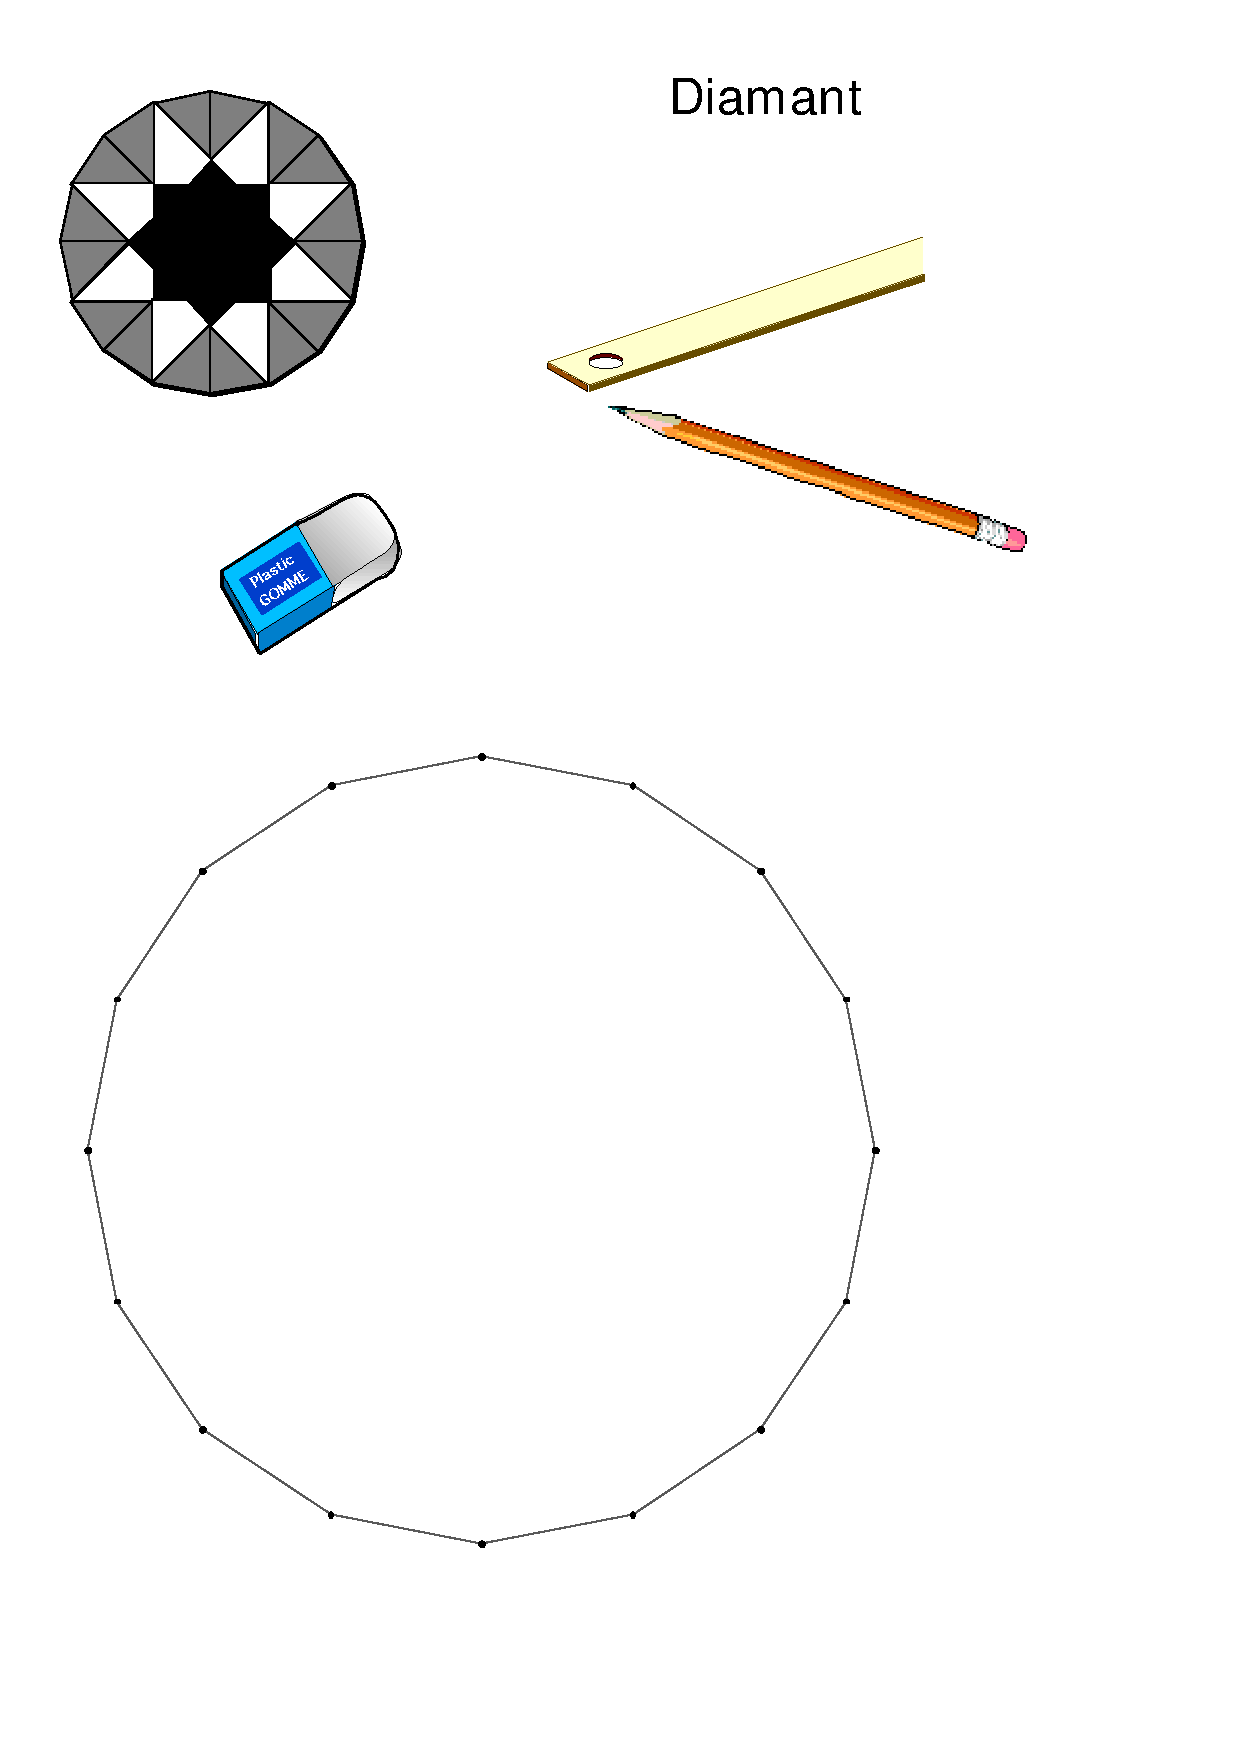
\includegraphics[width=0.3\linewidth]{sources/pages/1.2.1/2-diamant.pdf}}
    \caption{\hyperref[diamant]{Diamant}}
  \end{figure}

  \begin{figure}[H]
    \centering
    \fbox{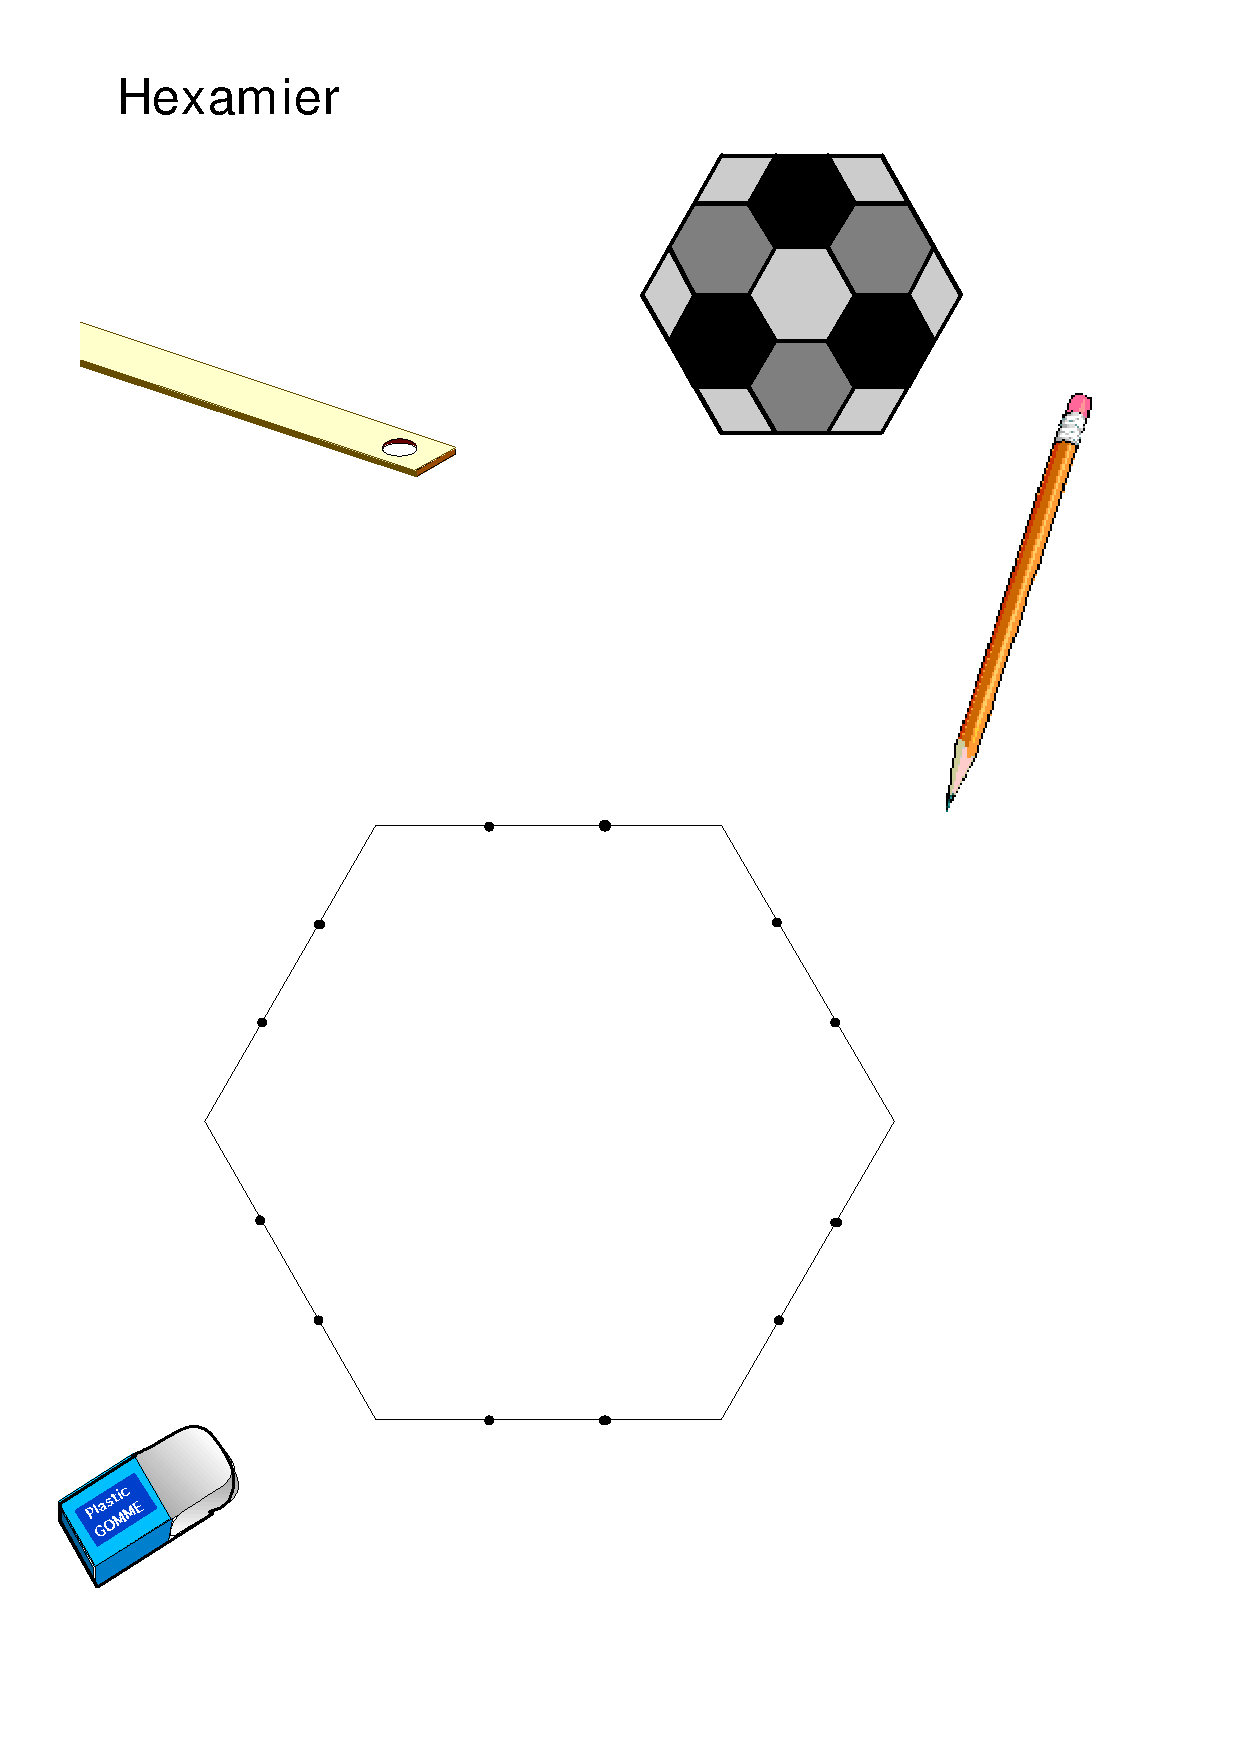
\includegraphics[width=0.3\linewidth]{sources/pages/1.2.1/3-hexamier.pdf}}
    \caption{\hyperref[hexamier]{Hexamier}}
  \end{figure}

  \begin{figure}[H]
    \centering
    \fbox{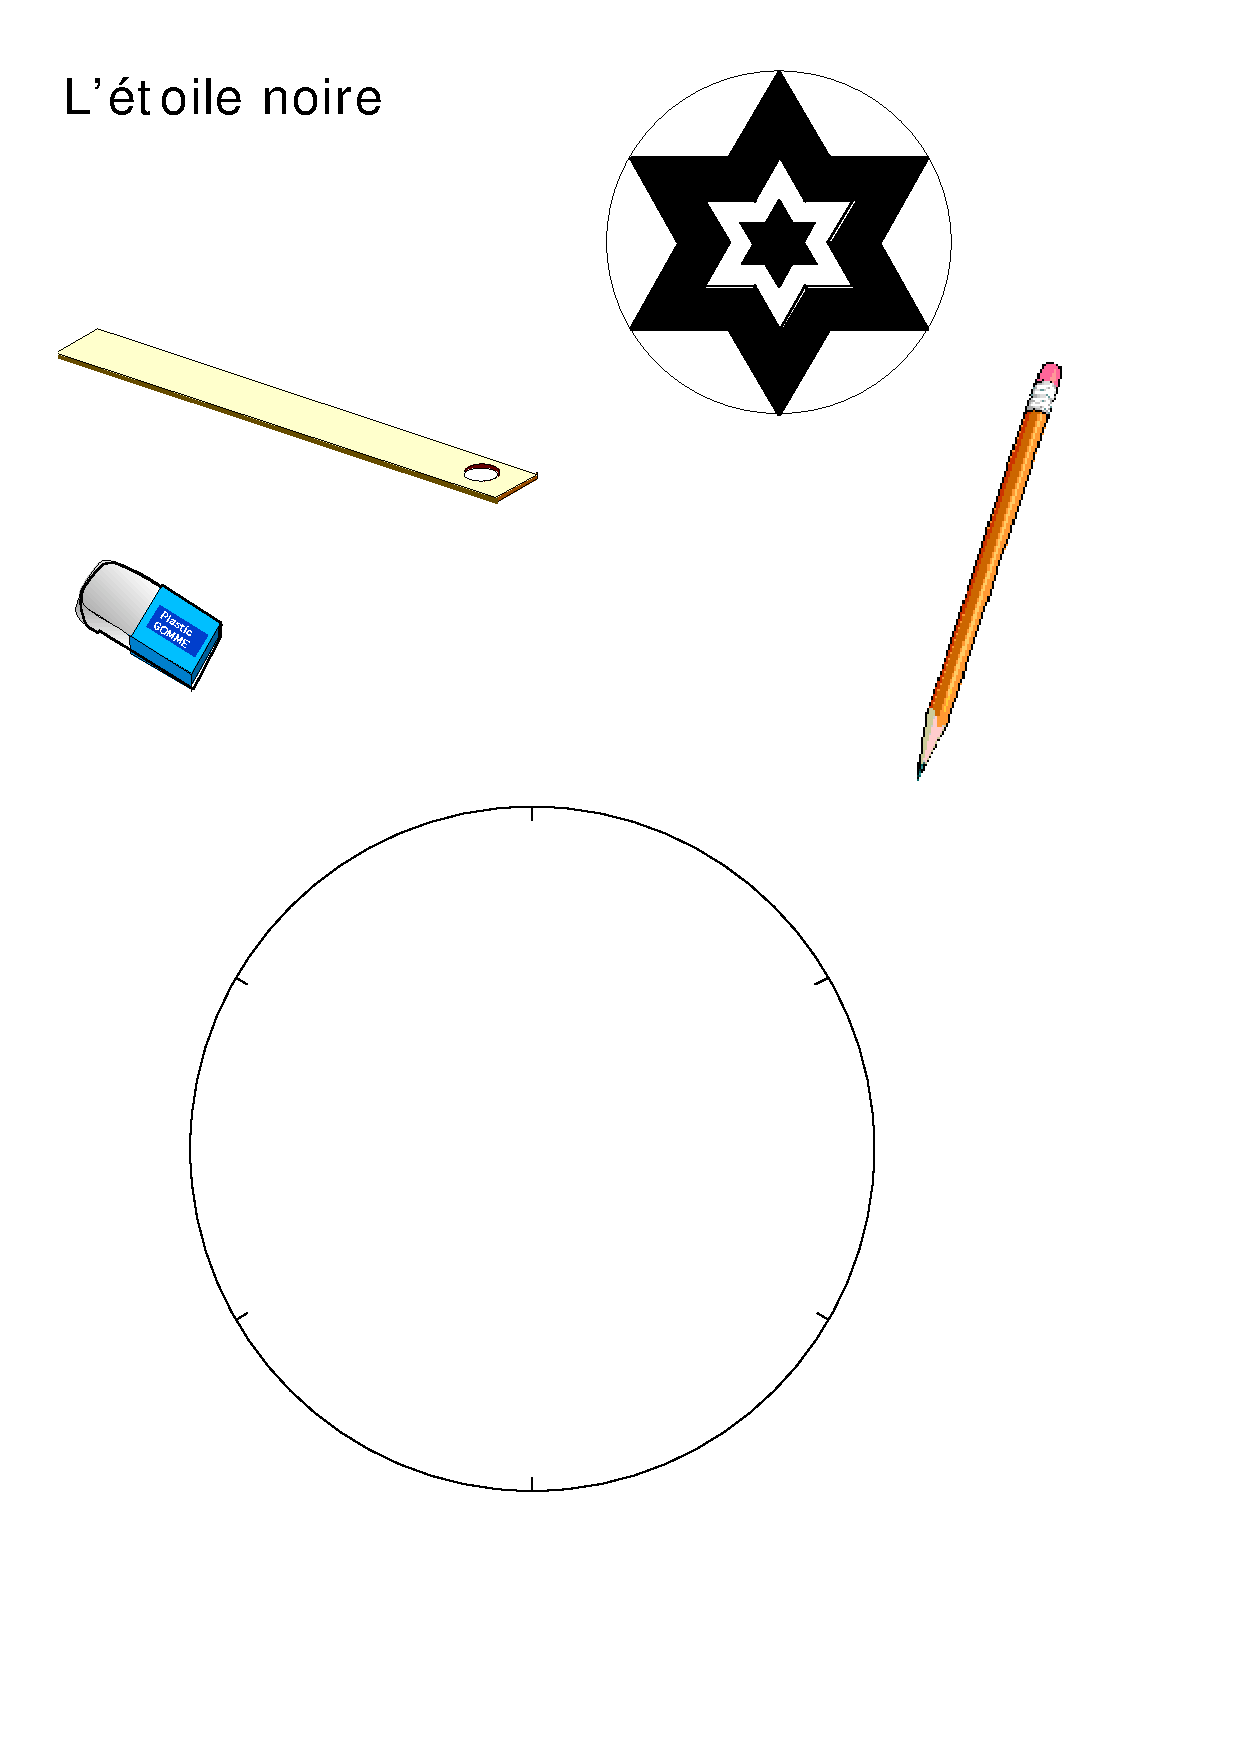
\includegraphics[width=0.3\linewidth]{sources/pages/1.2.1/4-etoilenoire.pdf}}
    \caption{\hyperref[etoilenoire]{Étoile noire}}
  \end{figure}

  \begin{figure}[H]
    \centering
    \fbox{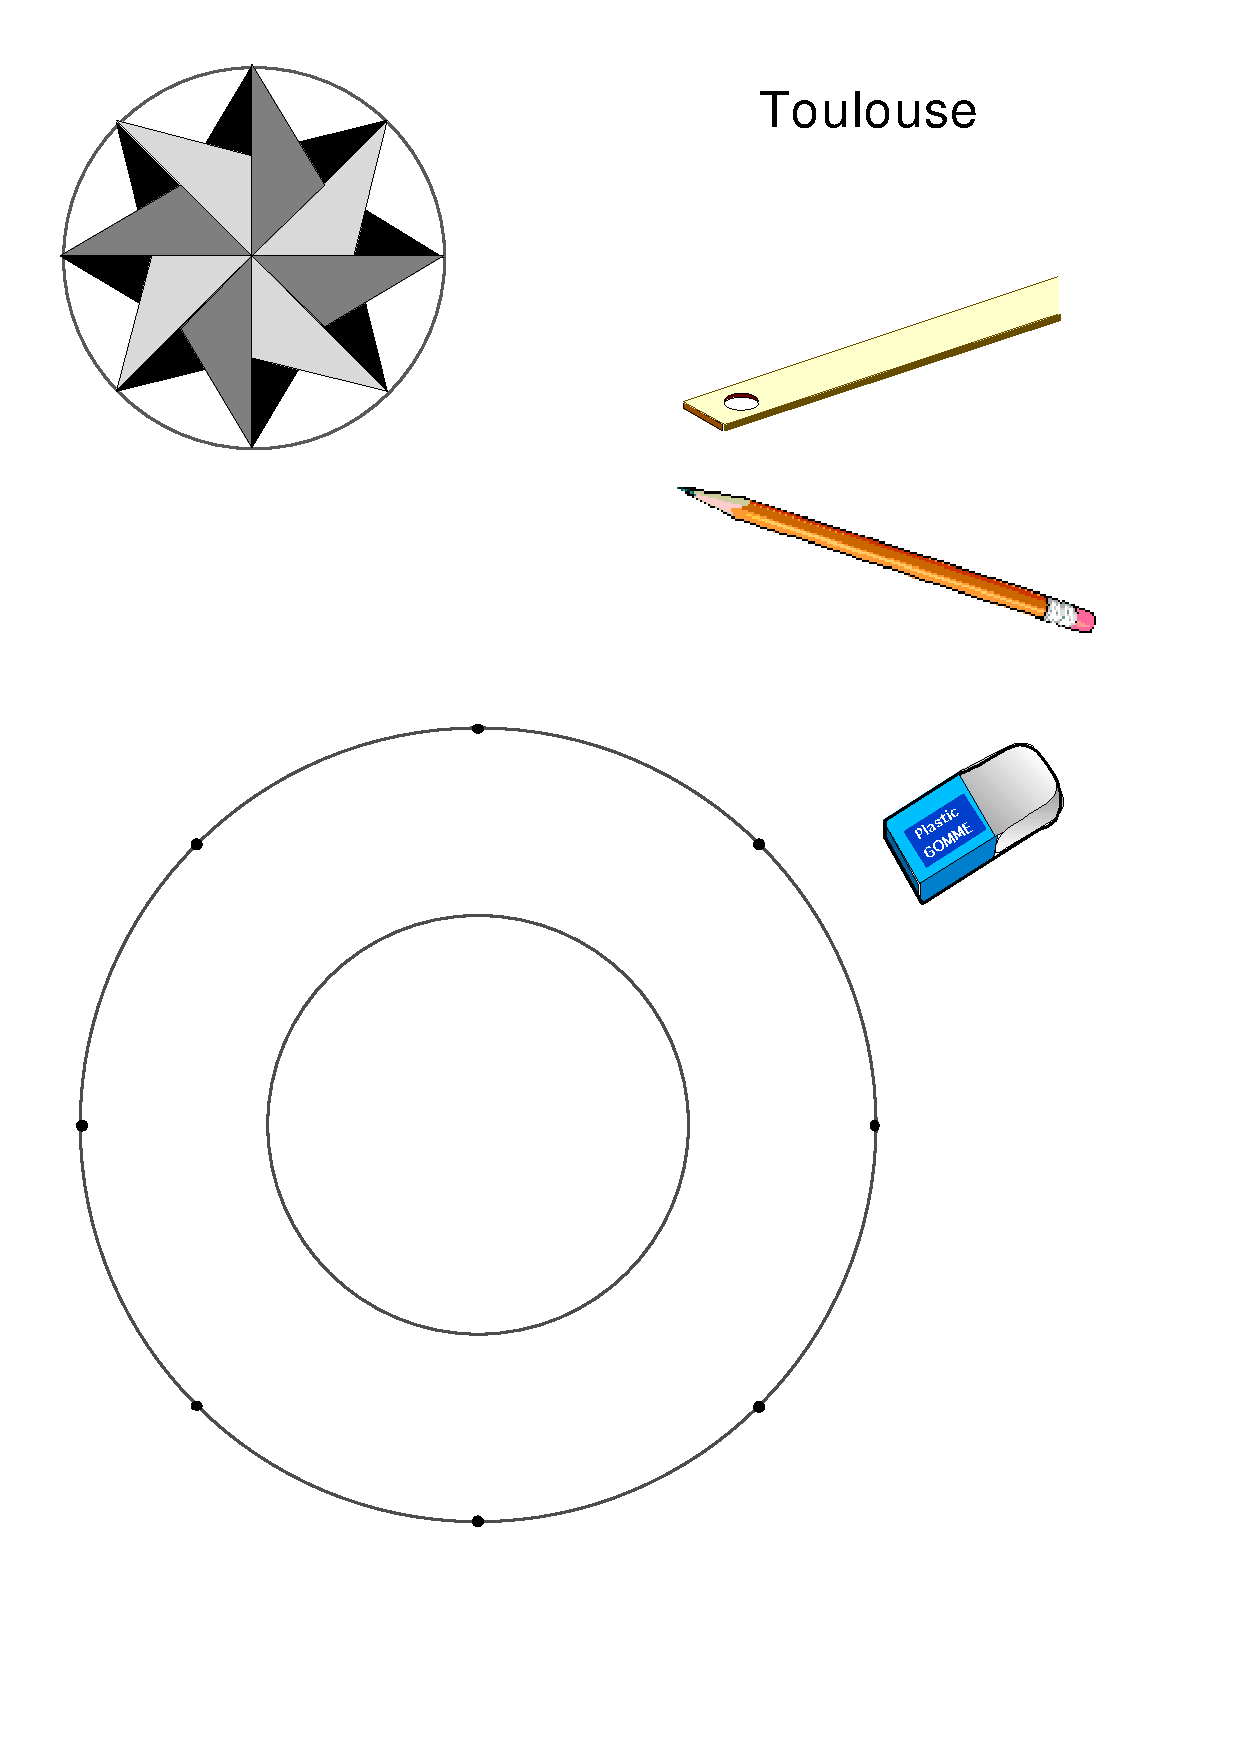
\includegraphics[width=0.3\linewidth]{sources/pages/1.2.1/5-toulouse.pdf}}
    \caption{\hyperref[toulouse]{Toulouse}}
  \end{figure}

  \begin{figure}[H]
    \centering
    \fbox{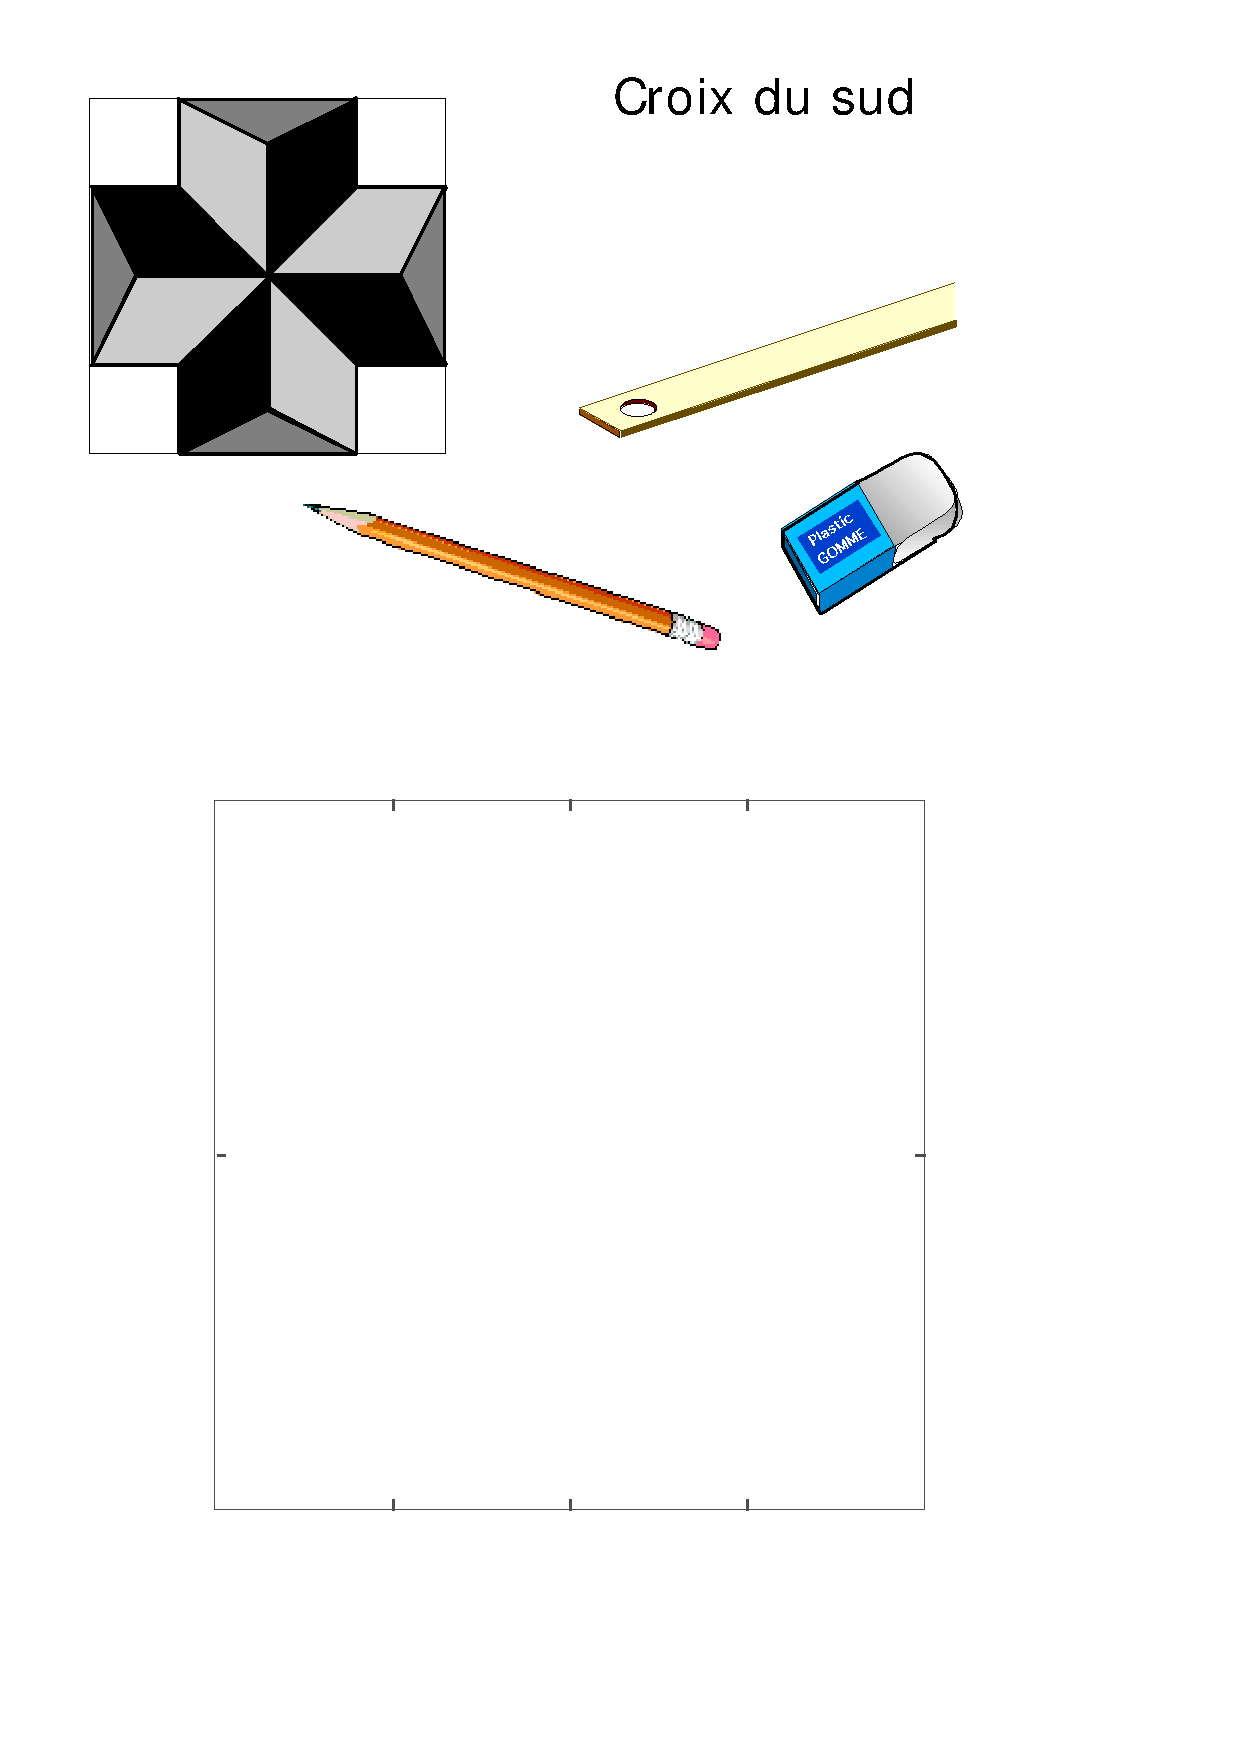
\includegraphics[width=0.3\linewidth]{sources/pages/1.2.1/6-croixdusud.pdf}}
    \caption{\hyperref[croixdusud]{Croix du sud}}
  \end{figure}

\end{multicols}

Les premiers dessins posent parfois de réelles difficultés aux élèves et il faut prendre le soin et le temps de bien leur faire comprendre les consignes. On peut pour cela faire des corrections avec un vidéo-projecteur.

Le coloriage des figures est important pour la suite et doit donc bien être réalisé.

Certains dessins peuvent faire l’objet de travaux à la maison (peut-être après un démarrage en classe).

On peut moduler le nombre de dessins à proposer en fonction de l’adresse manuelle des élèves, de leur capacité de soin, de leur bonne compréhension des consignes, etc.

\textit{Pour trouver d’autres dessins, se reporter aux brochures de l’Irem Paris-Nord : \og 130 Activités mathématiques au collège\fg{} et \og Papiers-Crayons \fg{}.}

\subsubsection{Activité Géogébra : Reproduire une figure}

Vous trouverez sur \textbf{Rubricamaths} de nombreux fichiers dans la partie : \href{http://www-irem.univ-paris13.fr/site_spip/spip.php?rubrique58}{Les bases de la géométrie avec Géogebra}.

L’élève doit reproduire le dessin présenté à partir des éléments de départ qui lui sont donnés. Pour cela, il utilise les outils du menu \og Lignes droites \fg{} : point, segment, droite, demi-droite, polygone, couleur, remplir, nommer, cacher/montrer.

Pour certains élèves, il est utile de donner un équivalent papier du travail demandé et d’autoriser ainsi une recherche antérieure ou simultanée avec la règle et le crayon.

La liberté qu’offre \textbf{Rubricamaths} dans le choix des figures proposées aux élèves permet d’individualiser le travail mais doit tout de même suivre une certaine logique.

Voici un exemple de progression :

\begin{multicols}{3}

  \begin{figure}[H]
    \centering
    \fbox{
\includegraphics[width=0.4\linewidth]{sources/img/1-1-sherif.png}}
    \caption{\href{http://www-irem.univ-paris13.fr/site_spip/IMG/ggb/sherif_multi-2.ggb}{Sherif}}
  \end{figure}

  \begin{figure}[H]
    \centering
    \fbox{
\includegraphics[width=0.4\linewidth]{sources/img/1-2-flash.png}}
    \caption{\href{http://www-irem.univ-paris13.fr/site_spip/IMG/ggb/flash_multi.ggb}{Flash}}
  \end{figure}

  \begin{figure}[H]
    \centering
    \fbox{
\includegraphics[width=0.4\linewidth]{sources/img/1-3-moulinette.png}}
    \caption{\href{http://www-irem.univ-paris13.fr/site_spip/IMG/ggb/moulinette_multi.ggb}{Moulinette}}
  \end{figure}

  \begin{figure}[H]
    \centering
    \fbox{
\includegraphics[width=0.4\linewidth]{sources/img/1-4-hextoile.png}}
    \caption{\href{http://www-irem.univ-paris13.fr/site_spip/IMG/ggb/hextoile_multi.ggb}{Hextoile}}
  \end{figure}

  \begin{figure}[H]
    \centering
    \fbox{
\includegraphics[width=0.4\linewidth]{sources/img/1-5-multiflash.png}}
    \caption{\href{http://www-irem.univ-paris13.fr/site_spip/IMG/ggb/multiflash_multi-2.ggb}{Multiflash}}
  \end{figure}

  \begin{figure}[H]
    \centering
    \fbox{
\includegraphics[width=0.4\linewidth]{sources/img/1-6-soissons.png}}
    \caption{\href{http://www-irem.univ-paris13.fr/site_spip/IMG/ggb/soissons_multi.ggb}{soissons}}
  \end{figure}

\end{multicols}

\textit{Shérif} et \textit{Flash} correspondent à l’initiation au travail.

Le choix de refaire \textit{Moulinette} est volontaire. Il doit permettre à l’élève de bien comprendre que les points nécessaires à la réalisation des polygones attendus sont des points d’intersection de lignes (segments) qui relient des points déjà existants. Ce premier dessin peut être \og assisté \fg{} en utilisant un vidéo-projecteur et en faisant voir, par un élève, au groupe comment obtenir un ou des sommets des ailes du moulin. On peut proposer une autre figure du même genre pour vérifier l’acquisition de ce principe.

La réalisation de tous ces dessins nécessite le tracé de lignes droites. Si les trois premiers dessins n’utilisent que l’outil \og segment \fg{}, il n’en va pas de même avec \textit{Hextoile} qui va exiger l’emploi de l’outil \og demi-droite \fg{} et \textit{Multiflash} l’usage de l’outil \og droite \fg{}.

Le dernier dessin \textit{Soissons} n’est là que pour les \og experts \fg{}, ceux qui, allant plus vite, finissent très rapidement les premières figures.

\subsubsection{Bilan}

\textbf{Notions rencontrées} : point, droite, segment, demi-droite.

\textbf{Vocabulaire complémentaire} : extrémités d’un segment, origine d’une demi-droite, points alignés.

Après les activités proposées, l’élève doit avoir compris la différence entre droite, demi-droite et segment. Il pourra exprimer (voire noter sur un cahier) ces différences en termes naïfs (qu’il n’est peut être pas utile de corriger). Il lui faut aussi retenir les mots de vocabulaire utilisés. On peut aussi lui faire comprendre que pour écrire symboliquement \og la doite passant par A et par B\fg{} ou \og le segment d’extrémités A et B\fg{} il va être nécessaire de différencier par un code l’arrêt (extrémités, origine) du non-arrêt de la ligne. Les élèves ne manquent pas d’imagination pour marquer cette différence ( ... et / par exemple). Il ne restera plus alors qu’à donner le code commun en expliquant ce qu’est une convention et à quoi elle sert.

%-------------------------------------------------------------------------------
\subsection{Droites perpendiculaires}

Les activités informatiques de cette partie sont accessibles sur Rubricamaths en suivant ce lien.

%-------------------------------------------------------------------------------
\subsection{Droites parallèles}
